\documentclass{beamer}

\usepackage{beamerthemesplit}
\usepackage{graphicx}

%\usetheme{}

\title{Vorstellung der UML-Diagramme}
\subtitle{Vorausversionen für die Implementierung von Kolejka}
\author{Ludwig und Robin}
\date{\today}

\begin{document}
\maketitle
\frame{\tableofcontents[currentsection]}

\section{Uebersicht}
\begin{frame}
	\frametitle{Übersichtsdiagramm erstellt mit plantuml}	
		    \begin{figure}[h!]
            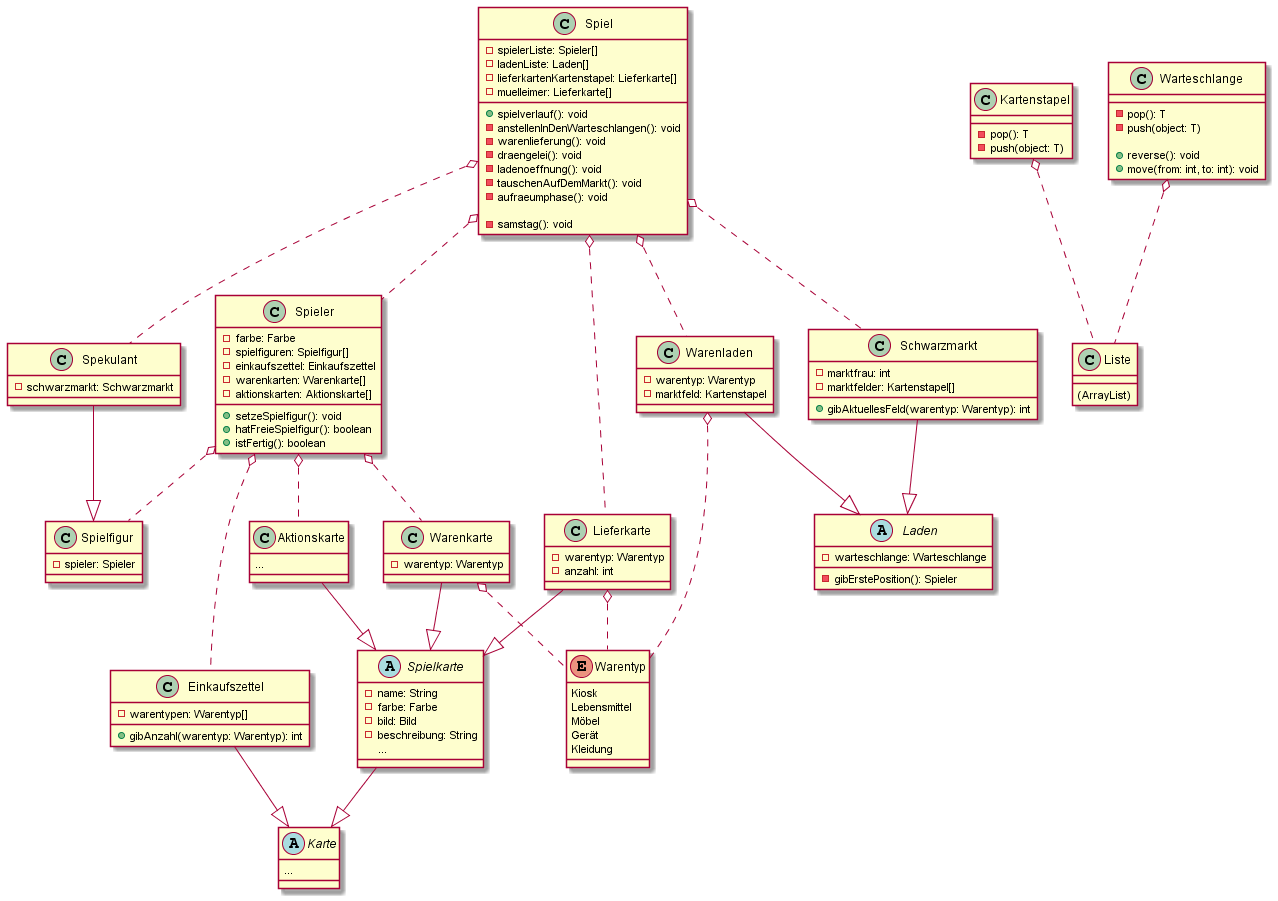
\includegraphics[width=0.7\linewidth]{../out/architecture_overview/architecture_overview.png}
            \caption{Übersicht der UML-Klasssen}
            \label{fig:boat1}
            \end{figure}
        
\end{frame}

\section{Verwendete Datenstrukuturen und deren Klassen}
\begin{frame}
	\frametitle{Noch ne Seite}	
		\begin{center}
			Noch eine tolle Seite.
		\end{center}
\end{frame}


\end{document}
